\chapter{Tecnologías utilizadas}
\label{cap:TecnologiasUtilizadas}

El capítulo actual se enfoca en detallar las tecnologías empleadas en la construcción y el despliegue del chatbot diseñado para asistir en terapias de reminiscencia. También se analizarán las herramientas y metodologías utilizadas en el proceso de desarrollo de prototipos, que se presenta en el capítulo \ref{cap:Desarrollo de prototipos}, así como su integración con los conceptos y conocimientos presentados en el estado de la cuestión.

En cada sección del capítulo, se llevará a cabo un análisis de las diferentes alternativas consideradas para la construcción de cada uno de los módulos que componen el chatbot. Desde la evaluación de diversas API's y bibliotecas de Procesamiento del Lenguaje Natural (PLN) hasta la exploración de las múltiples opciones disponibles para el desarrollo de la interfaz de usuario.

Esta metodología permitirá proporcionar un contexto completo y comprensible que facilitará la comprensión de las decisiones tomadas a lo largo del desarrollo del proyecto, como se detalla en el capítulo \ref{cap:Desarrollo de prototipos}. 
\newpage


\section{Bibliotecas de Procesamiento del Lenguaje en Python}

\subsection{NLTK}
La biblioteca NLTK (Natural Language Toolkit) \footnote{\href{https://www.nltk.org/}{Página oficial de NLTK}} ofrece una amplia gama de herramientas y recursos para tareas de PLN.

En primer lugar, NLTK permite realizar tareas como la tokenización y el  etiquetado POS (Part-Of-Speech tagging). Al utilizar las herramientas de tokenización, podemos dividir el texto en unidades más pequeñas, lo que facilita el análisis y la comprensión. El etiquetado POS asigna etiquetas gramaticales a cada palabra en el texto, lo que nos permite identificar la función de cada palabra en la oración. \\

\begin{lstlisting}[style=SpyderStyle, caption={Ejemplo de código en Python. Se pueden consultar más ejemplos en \cite{bird2009natural}}, captionpos=b, label={lst:python},breaklines = true]
	sentence = "Reminiscence Therapy involves the discussion of past activities using prompts like photos."
	tokens = nltk.word_tokenize(sentence)
	tagged = nltk.pos_tag(tokens)
	tagged[0:len(tagged)]
\end{lstlisting}

En este código $nltk$ tokeniza la oración introducida y etiqueta cada $token$ indicando la categoría sintáctica de cada $token$ como sigue:

\begin{itemize}
	\item NNP: Nombre propio singular
	\item NN: Nombre, singular o sustantivo singular
	\item VBZ: Verbo tercera persona del singular presente
	\item DT: Determinante
	\item IN: Preposición o oración subordinada
	\item JJ: Adjetivo
	\item NNS: Nombre plural 
	\item VBG: Verbo, gerundio o participio
	\item . : Signo de puntuación
\end{itemize}

\begin{lstlisting}[style=SpyderStyle, caption={Tokenización y etiquetado con nltk}, captionpos=b, label={lst:python},breaklines = true]
	>>>[('Reminiscence', 'NNP'), ('Therapy','NNP'), ('involves','VBZ'), ('the', 'DT'), ('discussion', 'NN'), ('of', 'IN'), ('past', 'JJ'), ('activities', 'NNS'), ('using', 'VBG'), ('prompts', 'NNS'), ('like', 'IN'), ('photos', 'NNS'), ('.', '.')]
	
\end{lstlisting}

Otras de las funcionalidades que nos permite esta biblioteca es el análisis sintáctico o lematización. Por ejemplo, nos permite la obtención de árboles sintácticos, lo que permite visualizar la estructura gramatical de las oraciones, facilita el análisis y la interpretación del texto. \\

\begin{figure}[h]
	\centering
	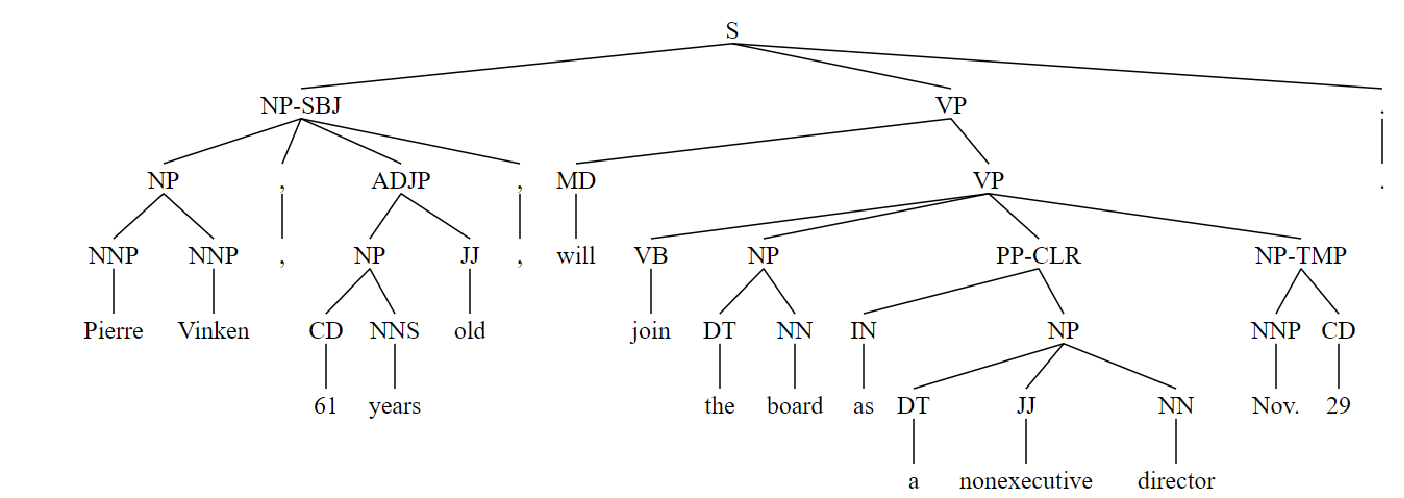
\includegraphics[width=0.9\textwidth]{Imagenes/arbolsintactico}
	\caption{Árbol sintáctico generado con nltk}
	\label{fig:2}
\end{figure}

\begin{lstlisting}[style=SpyderStyle, caption={Análisis sintáctico y lematización con nltk}, captionpos=b, label={lst:python},breaklines = true]
	entities = nltk.chunk.ne_chunk(tagged)
	nltk.download('treebank')
	from nltk.corpus import treebank
	t = treebank.parsed_sents('wsj_0001.mrg')[0]
	t
\end{lstlisting}


Además de estas características fundamentales, NLTK ofrece una serie de otras funcionalidades que amplían aún más su utilidad. Por ejemplo, incluye herramientas para la extracción de entidades nombradas, el análisis de sentimientos, la generación de texto y la traducción automática. Estas capacidades adicionales permiten abordar una amplia variedad de tareas en el procesamiento del lenguaje natural, desde la clasificación de texto hasta la generación de resúmenes automáticos y la traducción de idiomas. En resumen, NLTK es una herramienta invaluable para investigadores, estudiantes y profesionales que trabajan en el campo del PLN, ofreciendo una amplia gama de funcionalidades que facilitan el análisis, la comprensión y la manipulación del lenguaje humano.


\subsection{SpaCy}
\label{sec:Spacy}
SpaCy \footnote{\href{https://spacy.io/}{spaCy}}ofrece soporte para más de 25 idiomas y cuenta con 84 pipelines de entrenamiento. Utiliza el aprendizaje multi-tarea con modelos preentrenados como BERT, lo que permite un rendimiento avanzado en tareas de procesamiento del lenguaje natural. Sus componentes incluyen herramientas para el reconocimiento de entidades nombradas, etiquetado de partes del discurso, análisis de dependencias, segmentación de oraciones, clasificación de texto, lematización, análisis morfológico, vinculación de entidades y más.

\begin{lstlisting}[style=SpyderStyle, caption={Ejemplo de tokenización usando spaCy}, captionpos=b, label={lst:python},breaklines = true]
	import spaCy
	
	# Load English tokenizer, tagger, parser and NER
	nlp = spacy.load("en_core_web_sm")
	
	# Process whole documents
	text = ("Reminiscence Therapy involves the discussion of past activities using prompts like photos.")
	doc = nlp(text)
	
	# Analyze syntax
	print("Noun phrases:", [chunk.text for chunk in doc.noun_chunks])
	print("Verbs:", [token.lemma_ for token in doc if token.pos_ == "VERB"])
\end{lstlisting}

Este código carga el modelo preentrenado $"en\_core\_web\_sm"$ de spaCy, que incluye herramientas para tokenizar, etiquetar, analizar la sintaxis y reconocer entidades nombradas en textos en inglés. Luego, procesa el texto proporcionado y muestra las frases nominales identificadas utilizando la función $noun_chunks$ y los verbos lematizados utilizando la propiedad $lemma\_$. Este análisis gramatical permite identificar las partes clave del texto, como los sustantivos y las acciones descritas.

\begin{lstlisting}[style=SpyderStyle, caption={Resultado de tokenización usando spaCy}, captionpos=b, label={lst:python},breaklines = true]
	>>> Noun phrases: ['Reminiscence Therapy', 'the discussion', 'past activities', 'prompts', 'photos']
	Verbs: ['involve', 'use']
\end{lstlisting}

Además, es fácilmente ampliable con componentes y atributos personalizados, y es compatible con modelos personalizados en PyTorch, TensorFlow y otros frameworks. Spacy ofrece visualizadores integrados para la sintaxis y el reconocimiento de entidades nombradas, y facilita el empaquetado, despliegue y gestión de flujos de trabajo de modelos. Con su precisión rigurosamente evaluada y su robustez, Spacy es una herramienta poderosa y versátil para el procesamiento del lenguaje natural.

La biblioteca spaCy cuenta con diferentes componentes que interactúan entre sí esuchando la salida unos de otros para mejorar su procesamiento ($listener$). Además, existen una serie de reglas y dependencias entre los componentes. Por ejemplo, el módulo $atribute\_ruler$ indica proporciona reglas de etiquetado a $tagger$.

\begin{figure}[h]
	\centering
	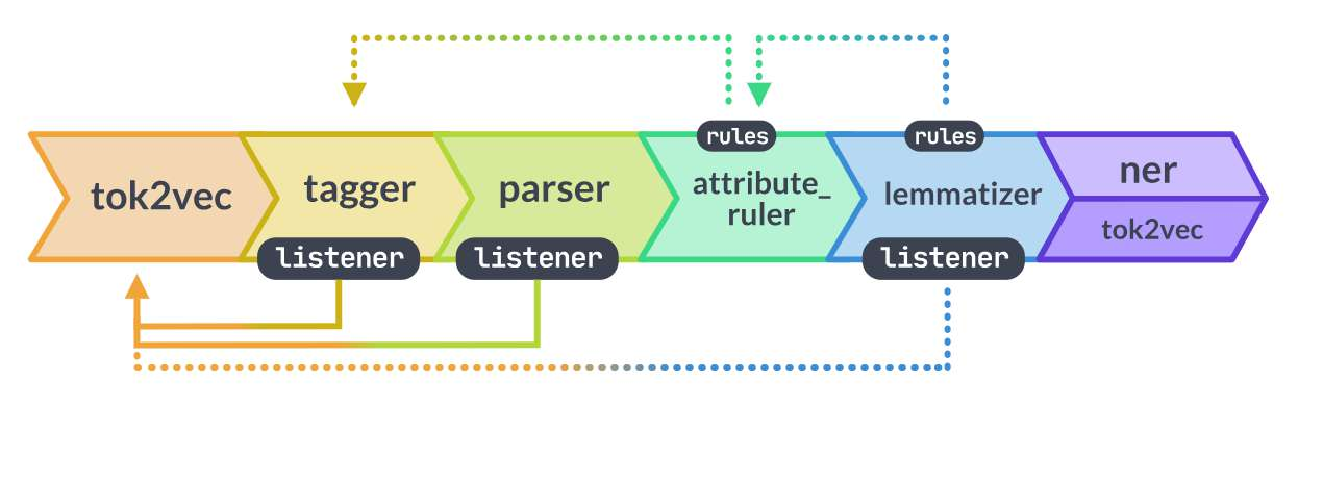
\includegraphics[width=0.9\textwidth]{Imagenes/spaCy}
	\caption{Árbol sintáctico generado con nltk}
	\label{fig:1}
\end{figure}

El gráfico representa la estructura de una tubería de procesamiento de lenguaje natural (NLP) en spaCy, mostrando la secuencia de componentes y sus interacciones.

\begin{itemize}
	\item tok2vec: Este componente convierte los tokens en vectores de palabras, que capturan el significado semántico de las palabras en el contexto de la oración.
	\item tagger: El $tagger$ asigna etiquetas gramaticales a cada token en el texto, como partes del discurso (POS).
	\item  parser: El analizador sintáctico analiza la estructura sintáctica del texto, identificando las relaciones de dependencia entre las palabras. 
	\item $attribute\_ruler$: Este componente aplica reglas para agregar atributos adicionales a los tokens, como excepciones de lema y POS, y manejar espacios en blanco de manera coherente.
	\item $lemmatizer$: El lematizador determina la forma base de cada palabra (su lema) en función de su contexto y su parte del discurso.
	\item $ner/tok2vec$: El componente de reconocimiento de entidades (NER) identifica entidades nombradas en el texto, como nombres de personas, lugares o organizaciones. En algunos modelos, este componente comparte la representación de vectores de palabras (tok2vec) con otros componentes para mejorar la coherencia y la precisión de las predicciones.
\end{itemize}
En resumen, este gráfico muestra cómo los componentes de spaCy interactúan entre sí para realizar tareas de procesamiento de lenguaje natural, aprovechando la información compartida y las reglas definidas para mejorar la precisión y la coherencia del análisis lingüístico.



\section{APIs de procesamiento del lenguaje}
\label{sec:apis}

Las APIs de procesamiento del lenguaje son conjuntos de herramientas y servicios que integran múltiples funcionalidades relacionadas con el PLN en sus aplicaciones y sistemas. Es decir, son herramientas que aúnan y ofrecen funcionalidades como el análisis de sentimientos, el reconocimiento de entidades o la tokenización. Frente a las bibliotecas y modelos presentados anteriormente presentan la ventaja de que se pueden usar sin necesidad de desarrollar desde cero algoritmos o modelos, lo que facilita su uso. Estas características hacen que este tipo de APIs sean comúnmente usadas en variedad de aplicaciones, desde chatbots hasta sistemas de recomendación. 

\subsection{Bard}
Bard es una API de procesamiento del lenguaje natural desarrollada por Google con el objetivo de ofrecer respuestas conversacionales coherentes y relevantes a través de interacciones de mensajes. Basada en LaMDA, un modelo de lenguaje experimental de Google, Bard compite directamente con ChatGPT en el campo del procesamiento del lenguaje natural, permitiendo realizar consultas y recibir respuestas sin necesidad de navegar por diferentes páginas web.

Google ha priorizado la accesibilidad y la transparencia en el desarrollo de Bard, ofreciendo modelos y recursos de PLN de código abierto que pueden ser utilizados y modificados por la comunidad. Inicialmente lanzado con un modelo reducido de LaMDA \ref{sec:LaMDA}, Bard busca ampliar su alcance y obtener comentarios para su mejora continua.

%Sustituir este ejemplo por otro que encuentre en internet ya que este lo he puesto en el desarrollo de prototipos
\begin{figure}[h]
	\centering
	\begin{verbatim}
prompt = "A partir del texto a continuación, que contiene información
 sobre una persona y damelo en una lista info donde
 info[nombre]:valor_atributo."

texto = "Hola mi nombre es Marta, tengo 22 años y soy de Zaragoza"
>> **Info[nombre:Marta;edad:22;ciudad:Zaragoza]** 
¿Hay algo más que pueda hacer por ti?
	\end{verbatim}
	\caption{ Ejemplo de uso de BARD.}
	\label{fig:ejemploBARD}
\end{figure}




Cómo se puede ver en el ejemplo, Bard es capaz de analizar la información proporcionada y generar respuestas coherentes y formateadas según las especificaciones dadas. Gracias a su capacidad para comprender el contexto y generar texto de manera precisa, Bard es una herramienta valiosa para tareas que requieren PLN, como la generación de respuestas conversacionales. Todo ello lo convierte en una opción ideal para una amplia gama de aplicaciones, desde chatbots hasta sistemas de asistencia virtual. 

Sin embargo, Bard ya no está disponible. En diciembre de 2023, Google fortaleció la capacidad de Bard al incorporar Gemini Pro en inglés, brindando habilidades más avanzadas de comprensión, razonamiento, resumen y codificación. Más adelante, en febrero de 2024, se anunció la expansión de Gemini Pro a más de 40 idiomas y se oficializó el cambio de nombre de Bard a Gemini, lo que implicó descartar el primer modelo del proyecto desarrollado en Bard debido a la indisponibilidad de Gemini en España en ese momento.

\subsection{Gemma}

Gemma es una API de PLN desarrollada por OpenAI. Utiliza modelos de lenguaje basados en la arquitectura GPT (Generative Pre-trained Transformer) para una variedad de tareas de PLN, como generación de texto, análisis de sentimientos, clasificación de texto, y más. Gemma se destaca por su capacidad para generar texto coherente y de alta calidad en una variedad de estilos y tonos, así como por su facilidad de uso y su API intuitiva.

Una de las principales ventajas de Gemma es su rendimiento en tareas de generación de texto, donde ha establecido nuevos estándares de calidad y coherencia en muchos casos. Además, Gemma ofrece modelos pre-entrenados en varios dominios y lenguas, lo que facilita su integración en una variedad de aplicaciones de PLN. Sin embargo, debido a su enfoque en modelos de última generación, Gemma puede requerir recursos computacionales significativos y puede ser más difícil de entender y utilizar para usuarios principiantes en PLN.


En primer lugar, estos modelos se trabajaron en Google Collaborate aumentando el número de GPUs. De esta forma gemma tiene un buen comportamiento y genera respuestas adecuadas y coherentes. En concreto, una respuesta generada por \textit{gemma-7b} sería la siguiente.
\begin{figure}[h]
	\centering
	\begin{verbatim}
prompt =gemma_lm.generate("What is the meaning of life?",
 max_lenght = 64)
 >>> The question is one of the most important questions in the world.
  It's the question that has been asked by philosophers, theologians and
  scientist for centuries. And it's the question that has been asked by
  people who are looking for answer to their own lives. 
	\end{verbatim}
	\caption{ Ejemplo de uso de GEMMA.}
	\label{fig:ejemploBARD}
\end{figure}
Sin embargo, las limitaciones propias de Google Collaborate no permitían en la versión gratuita aumentar el número de GPUs de forma frecuente y en consecuencia tuve que estudiar el modelo en otro entorno. Para ejecutarlo de forma local y obtener un buen comportamiento es necesario instalar Linux y descargar el modelo de Hugging face. 

Aunque \textit{gemma-2b} en la versión local instalada desde Hugging Face en Linux tiene un buen comportamiento, genera respuestas incoherentes que hacen de este modelo poco útil para nuestro proyecto. La versión \textit{gemma-7b} genera respuestas mucho mejores pero tiene la enorme desventaja de que ocupa una gran cantidad de espacio en memoria.

\subsection{GPT API}

GPT API es una API de PLN desarrollada por OpenAI. Utiliza modelos de lenguaje basados en la arquitectura GPT (Generative Pre-trained Transformer) para una variedad de tareas de PLN, como generación de texto, análisis de sentimientos, clasificación de texto, y más. GPT API se destaca por su capacidad para generar texto coherente y de alta calidad en una variedad de estilos y tonos, así como por su facilidad de uso y su API intuitiva.

Una de las principales ventajas de GPT API es su rendimiento en tareas de generación de texto, donde ha establecido nuevos estándares de calidad y coherencia en muchos casos. Además, GPT API ofrece modelos pre-entrenados en varios dominios y lenguas, lo que facilita su integración en una variedad de aplicaciones de PLN. Sin embargo, debido a su enfoque en modelos de última generación, GPT API puede requerir recursos computacionales significativos y puede ser más difícil de entender y utilizar para usuarios principiantes en PLN.

Sin embargo para obtener el comportamiento que se necesitaba en este trabajo debía ser entrenada, y debido a las limitaciones hardware esto suponía una cantidad de tiempo inviable. 

\subsection{Rasa}
\label{subsec:rasa}
Entre las opciones que se barajaron para seguir desarrollando el proyecto se encuentra Rasa. Rasa es una plataforma de código abierto diseñada para el desarrollo de chatbots y asistentes virtuales conversacionales. Utilizando técnicas de procesamiento de lenguaje natural y aprendizaje automático, Rasa permite a los desarrolladores crear sistemas de diálogo inteligentes y personalizados. Una de las principales ventajas de Rasa es su flexibilidad y personalización, ya que los desarrolladores tienen control total sobre el comportamiento y la lógica de sus chatbots. Además, Rasa proporciona herramientas robustas para la gestión del diálogo, la comprensión del lenguaje natural y la integración con otros sistemas. Sin embargo, una posible desventaja de Rasa es su curva de aprendizaje, ya que requiere un conocimiento sólido de PLN y aprendizaje automático para aprovechar al máximo su potencial. Además, debido a su naturaleza de código abierto, puede requerir más tiempo y recursos para implementar y mantener en comparación con otras soluciones comerciales. Sin embargo, aunque rasa no es la API más potente en cuánto a generación de texto, tiene numerosas aplicaciones que resultan interesantes. 

\section{Gemini}
\label{sec:gemini}
%De aqui quiero sacar varias páginas, ver el tutorial y ir metiendo todo

Gemini es una API de procesamiento del lenguaje natural (PLN) desarrollada por Google que permite a los usuarios interactuar con modelos de lenguaje avanzados para generar texto coherente y relevante en respuesta a consultas y solicitudes. Utiliza modelos de lenguaje de última generación entrenados por Google, que son capaces de comprender y generar texto en varios idiomas y contextos. Los usuarios pueden enviar texto de entrada a través de la API y recibir respuestas generadas por los modelos de Gemini. Ofrece varios modelos para satisfacer diferentes necesidades y casos de uso, entre los que se encuentran:
\begin{itemize}[label=$\bullet$, leftmargin=*]
	\item \textbf{gemini-pro}: Optimizado para entradas de texto.
	\item \textbf{gemini-pro-vision}: Optimizado para entradas multimodales de texto e imágenes.
\end{itemize}

Gemini puede utilizarse para una variedad de aplicaciones, incluyendo generación de texto a partir de entradas bien sean de texto, o imágenes, conversaciones de varios turnos (chats) o para la obtención de embeddings para modelos del lenguaje. 

Para configurarlo, en primer lugar hay que ejecutar el programa mibot.py estando en telegram en la conversaa conversación de telegram el comando /start para comenzar la conversación y ya. 

Sin embargo, y pese a las grandes funcionalidades de todas estas alternativas nos hemos decantado por hacer una interfaz con telegram desarrollando nuestro propio chatbot usando rasa. 

Para desarrollar el chatbot de telegram me he decantado por usar la interfaz de telegram para la cuál se necesita la API de Rasa. Las principales ventajas que ofrece esta herramienta es la facilidad del manejo de la interfaz pues telegram es una herramienta muy conocida con la que los terapeutas pueden estar más familiarizados. Además, esto nos permite también usar la versión del chatbotyayo para móvil. 

\subsection{Procesamiento de texto}

El modelo más apropiado para el procesamiento de texto es $gemini-pro$. La estructura de las respuestas de este modelo es la siguiente. 

\begin{lstlisting}[style=SpyderStyle, caption={Estructura de una respuesta de Gemini}, captionpos=b, label={lst:python},breaklines = true]
	{
		"candidates": [
		{
			"content": {
				"parts": [
				{
					"text": string
				}
				]
			},
			"finishReason": enum (FinishReason),
			"safetyRatings": [
			{
				"category": enum (HarmCategory),
				"probability": enum (HarmProbability),
				"blocked": boolean
			}
			],
			"citationMetadata": {
				"citations": [
				{
					"startIndex": integer,
					"endIndex": integer,
					"uri": string,
					"title": string,
					"license": string,
					"publicationDate": {
						"year": integer,
						"month": integer,
						"day": integer
					}
				}
				]
			}
		}
		],
		"usageMetadata": {
			"promptTokenCount": integer,
			"candidatesTokenCount": integer,
			"totalTokenCount": integer
		}
	}
\end{lstlisting}

\begin{itemize}
	\item \textbf{text}	El texto generado.
	\item \textbf{finishReason}	El motivo por el que el modelo dejó de generar tokens. Si está vacío, el modelo no dejó de generar los tokens. El motivo puede ser cualquiera de los siguientes:
	\begin{enumerate}
		\item $FINISH\_REASON\_UNSPECIFIED$: no se especifica el motivo de finalización.
		\item $FINISH\_REASON\_STOP$: punto de detención natural del modelo o secuencia de detención proporcionada.
		\item $FINISH\_REASON\_MAX\_TOKENS$: se alcanzó la cantidad máxima de tokens especificada en la solicitud.
		\item $FINISH\_REASON\_SAFETY$: la generación del token se detuvo porque la respuesta se marcó por motivos de seguridad. Ten en cuenta que Candidate.content está vacío si los filtros de contenido bloquean el resultado.
		\item $FINISH\_REASON\_RECITATION$: la generación del token se detuvo porque la respuesta se marcó para citas no autorizadas.
		\item $FINISH\_REASON\_OTHER$: todos los demás motivos que detuvieron el token
	\end{enumerate}
	
	\item \textbf{category}	La categoría de seguridad para la que se configura un umbral. Los valores aceptables son los siguientes:
	Haz clic para expandir las categorías de seguridad
	\begin{enumerate}
		\item $HARM\_CATEGORY\_SEXUALLY\_EXPLICIT$
		\item $HARM\_CATEGORY\_HATE\_SPEECH$
		\item $HARM\_CATEGORY\_HARASSMENT$
		\item $HARM\_CATEGORY\_DANGEROUS\_CONTENT$
	\end{enumerate}
	\item \textbf{probability}	Los niveles de probabilidad de daños en el contenido.
	\begin{enumerate}
		\item $HARM\_PROBABILITY\_UNSPECIFIED$
		\item $NEGLIGIBLE$
		\item $LOW$
		\item $MEDIUM$
		\item $HIGH$
	\end{enumerate}
	\item \textbf{blocked}	Una marca boolean asociada con un atributo de seguridad que indica si la entrada o salida del modelo se bloqueó. Si blocked es true, el campo errors en la respuesta contiene uno o más códigos de error. Si blocked es false, la respuesta no incluye el campo errors.
	\item \textbf{startIndex}	Un número entero que especifica dónde comienza una cita en el contenido.
	\item \textbf{endIndex}	Un número entero que especifica dónde termina una cita en content.
	\item \textbf{url}	Es la URL de una fuente de cita. Los ejemplos de una fuente de URL pueden ser un sitio web de noticias o un repositorio de GitHub.
	\item \textbf{title}	Es el título de una fuente de cita. Los ejemplos de títulos de origen pueden ser los de un artículo de noticias o un libro.
	\item \textbf{license}	Es la licencia asociada con una cita.
	\item \textbf{publicationDate}	La fecha en que se publicó una cita. Sus formatos válidos son YYYY, YYYY-MM y YYYY-MM-DD.
	\item \textbf{promptTokenCount}	Cantidad de tokens en la solicitud.
	\item \textbf{candidatesTokenCount}	Cantidad de tokens en las respuestas.
	\item \textbf{totalTokenCount}	Cantidad de tokens en la solicitud y las respuestas.
\end{itemize} 

\subsection{Procesamiento de imágenes}
%https://developers.google.com/solutions/content-driven/ai-images?continue=https%3A%2F%2Fdevelopers.google.com%2Flearn%2Fpathways%2Fsolution-ai-gemini-images&hl=es-419#article-https://developers.google.com/solutions/content-driven/ai-images&hl=es-419

Los mensajes multimodales son instrucciones que utilizan modelos avanzados de lenguaje y admiten diferentes tipos de entradas, como texto e imágenes. Al combinar múltiples formatos de entrada, estos mensajes permiten una amplia gama de aplicaciones, como la clasificación de imágenes, el reconocimiento de escritura a mano, la traducción y otras tareas creativas.

En esta sección, exploraremos los tipos de instrucciones que pueden generarse al ingresar tanto imágenes como texto en el modelo Gemini. A través de ejemplos interesantes, veremos cómo este modelo puede procesar esta información multimodal y producir respuestas en forma de texto.

En la actualidad, Gemini \footnote{\href{https://developers.google.com/solutions/content-driven/ai-images}{Página oficial de Google con más ejemplos}} tiene la capacidad de procesar solicitudes que combinan texto e imagen como entrada, y luego generar respuestas basadas únicamente en texto. El texto puede utilizarse para contextualizar la imagen o para solicitar al modelo que opere y genere una respuesta relacionada con la imagen.

Un ejemplo muy simple que destaca la capacidad del LLM de reconocer la existencia de algo en una imagen o no y de responder al desarrollador de manera booleana, es el que muestra la figura \ref{fig:gemini-1}. Este enfoque puede ser útil en la detección de contenido específico.

\begin{figure}[h]
	\centering
	
\includegraphics[width=0.6\textwidth]{Imagenes/ImagenesGemini/gemini-2}
	\caption{Imagen de entrada a Gemini en el primer ejemplo}
	\label{fig:gemini-1}
\end{figure}
 
\begin{verbatim}
	>>> ¿En esta imagen aparece un gato?
	Respuesta de Gemini:  True
\end{verbatim}

Otro ejemplo es el asociado a la figura, \ref{fig:gemini-9}. Aquí vemos el poder de Gemini para narrar historias y formas más creativas de usar la IA generativa. 

\begin{figure}[h]
	\centering
	
\includegraphics[width=0.4\textwidth]{Imagenes/ImagenesGemini/gemini-9}
	\caption{Imagen de entrada a Gemini en el segundo ejemplo}
	\label{fig:gemini-9}
\end{figure}

\begin{verbatim}
	>>> Escribe un haiku sobre esta foto
	Respuesta de Gemini: 
	 
	Un banco junto al lago,
	
	Una vista de las montañas más allá,
	
	Un momento de paz.
\end{verbatim}
Finalmente, un ejemplo en el que se combinan varias habilidades de Gemini es el que se muestra en la figura \ref{fig:gemini-10}. No solo reconoce las formas, sino que también entiende que, si bien las formas son levemente dibujadas, están destinadas a ser formas distintas vinculadas matemáticamente con atributos específicos (p.ej., 3 lados, 4 lados, 5 lados).

Además, la presencia del signo de interrogación no confunde a Gémini en su interpretación de la progresión lógica de las formas geométricas. En cambio, Gemini identifica que esta es una progresión matemática de 3, 4 a 5 y que, por lo tanto, la última forma tendría 6 lados y propone un hexágono.

\begin{figure}[h]
	\centering
	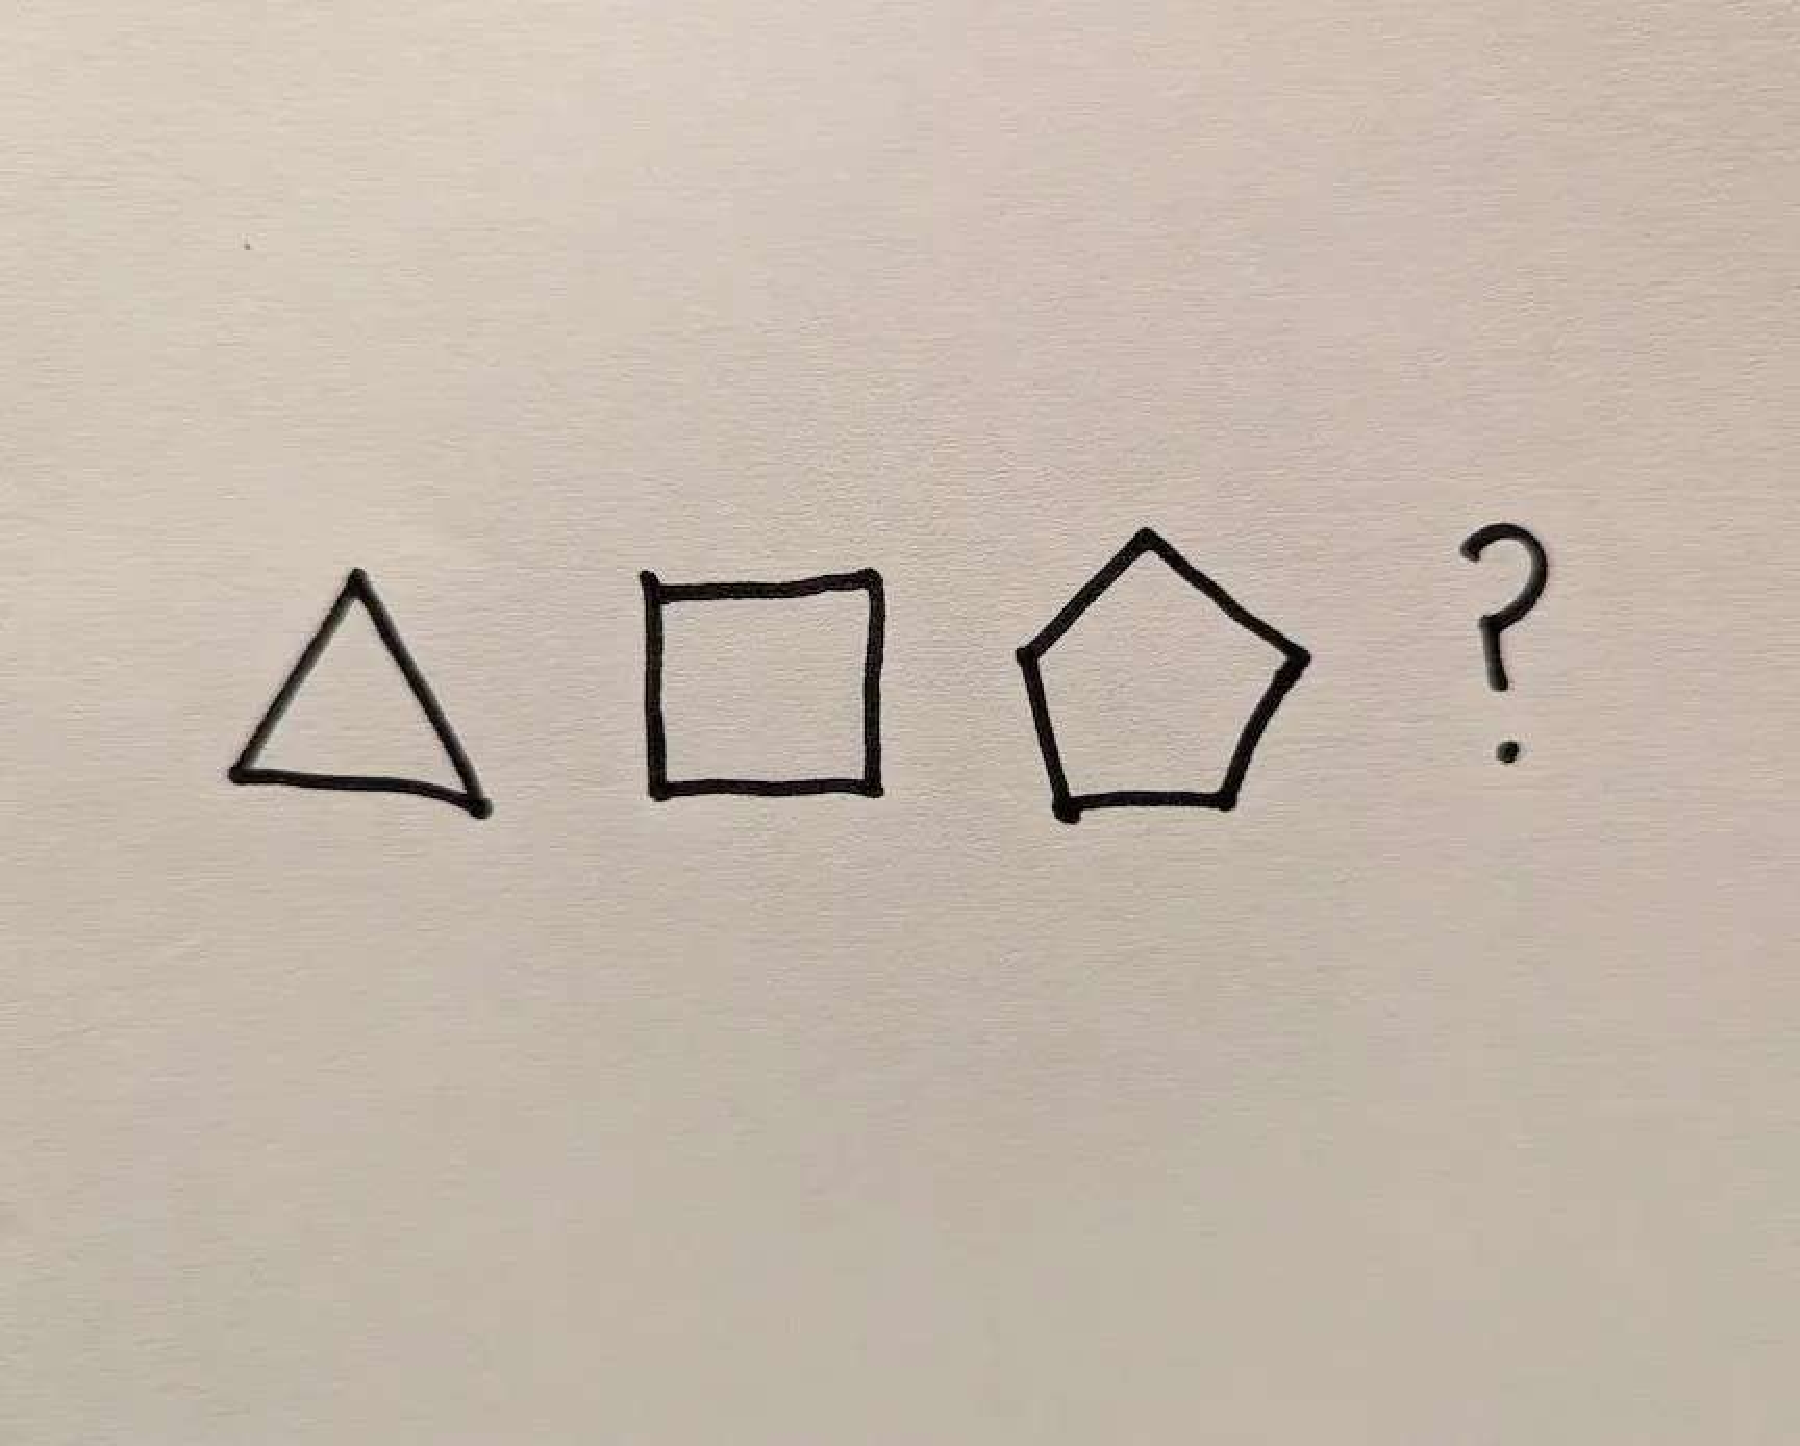
\includegraphics[width=0.6\textwidth]{Imagenes/ImagenesGemini/gemini-10}
	\caption{Imagen de entrada a Gemini en el ejemplo}
	\label{fig:gemini-10}
\end{figure}
\begin{verbatim}
	>>> ¿Qué sigue? Explica tu razonamiento
	Respuesta de Gemini: El triángulo tiene 3 lados, el cuadrado tiene 4 lados
	 y el pentágono tiene 5 lados. El número de lados aumenta en 1 para cada
	  forma. Por lo tanto, la siguiente forma debería tener 6 lados, que es un
	   hexágono.
\end{verbatim}

\section{Almacenamiento de la información}	
\subsection{JSON}
El JSON, acrónimo de JavaScript Object Notation, es un formato ligero para estructurar datos que se asemeja a los mapas en la programación. Está diseñado para representar datos de manera legible para las máquinas y fácilmente interpretable por los humanos. Se utiliza ampliamente en el intercambio de datos entre aplicaciones web y en el manejo de respuestas de API. El formato JSON consta de pares de clave-valor, donde las claves son únicas y los valores pueden ser cadenas, booleanos, números, objetos JSON o matrices JSON.

En Python, el formato de datos más cercano a JSON es el diccionario. El módulo `json` de Python permite la conversión entre diccionarios, cadenas JSON y archivos JSON. Para leer un archivo JSON en Python, se utiliza la función \textit{json.load()} para cargar los datos del archivo en un diccionario. Para leer una cadena JSON en Python, se utiliza la función  \textit{json.loads()} para analizar la cadena y convertirla en un diccionario.

Para escribir datos en un archivo JSON, se utiliza la función \textit{json.dump()} para escribir un diccionario en un archivo JSON. También se puede utilizar la función \textit{json.dumps()} para convertir un diccionario en una cadena JSON y luego escribir esa cadena en un archivo. Ambas funciones permiten especificar la indentación para formatear el archivo JSON de manera legible. El módulo \textit{json} proporciona una forma conveniente de manipular datos JSON en Python, facilitando el intercambio de datos entre aplicaciones y su almacenamiento en archivos.

\subsection{RDF}

%Las tripletas RDF (Resource Description Framework) son una estructura de datos fundamental en la web semántica para representar información en forma de sujetos, predicados y objetos. Cada tripleta consiste en un sujeto que es una entidad, un predicado que describe la relación entre el sujeto y el objeto, y un objeto que puede ser una entidad o un valor. Por ejemplo, en la tripleta "Gato - es_un - Animal", "Gato" es el sujeto, "es_un" es el predicado y "Animal" es el objeto.

Estas tripletas RDF se utilizan para almacenar información de manera estructurada y semántica, lo que permite una representación más rica y significativa de los datos en la web. A través de vocabularios y ontologías, como RDF Schema (RDFS) y Web Ontology Language (OWL), se establecen relaciones y significados precisos entre los términos utilizados en las tripletas RDF.

Las tripletas RDF son ampliamente utilizadas en la web semántica para diversas aplicaciones, como la descripción de recursos y metadatos en la web, la integración de datos de diferentes fuentes, la creación de motores de búsqueda más inteligentes y la construcción de sistemas de recomendación personalizados. Además, RDF proporciona un marco estándar y flexible para representar conocimiento y facilita la interoperabilidad entre diferentes sistemas y aplicaciones en la web.

	
El Framework de Descripción de Recursos (RDF, por sus siglas en inglés) es un lenguaje de propósito general orientado a la representación de información en la web. Su uso se centra en el desarrollo de la web semántica, y tiene como finalidad describir los recursos de la misma de una manera no orientada a la legibilidad por parte de un humano, sino a la computación de la información contenido por un ordenador.

La web semántica es un proyecto de futuro en el que la información web tiene un significado exactamente definido y puede ser procesado por ordenadores. Por lo tanto, los ordenadores pueden integrar y usar la información disponible en la web. Más información sobre la web semántica puede ser encontrada en \cite{iswc2007}.

RDF está considerado como un lenguaje de metadatos, o "datos sobre datos", ya que con los símbolos de RDF añadimos metainformación a los datos que realmente nos interesan para poder interpretarlos de una manera exacta, es decir, de aquella que el autor de los datos (o, al menos, del autor del marcado RDF sobre estos datos) quería que estos fuesen interpretados.

RDF define los recursos mediante descripciones de los mismos, como puede verse en el listado \ref{fig:ejemploRDF1}. Puede encontrarse más información sobre la manera de la tecnología RDF de describir estos recursos en \cite{champin2002rdf}.

\begin{figure}[h]
	\centering
	\begin{verbatim}
		<rdf:Description
		rdf:about="http://www.recshop.fake/cd/Empire Burlesque">
		<cd:artist>Bob Dylan</cd:artist>
		<cd:country>USA</cd:country>
		<cd:company>Columbia</cd:company>
		<cd:price>10.90</cd:price>
		<cd:year>1985</cd:year>
		</rdf:Description>
	\end{verbatim}
	\caption{ Ejemplo de un recurso RDF.}
	\label{fig:ejemploRDF1}
\end{figure}


RDF no define clases de datos específicas para las aplicaciones. En vez de esto, el estándar RDF dispone de RDF Schema. Estos documentos definen nuevas clases, y relaciones entre ellas (herencia, agregación) de una manera muy similar a aquella con la que se acostumbra en la programación orientada a objetos. En la Figura \ref{fig:ejemploRDF2} podemos ver un ejemplo de un RDF Schema.

\begin{figure}[t]
	\centering
\begin{verbatim}
	<?xml version="1.0"?>
	<rdf:RDF
	xmlns:rdf= "http://www.w3.org/1999/02/22-rdf-syntax-ns#"
	xmlns:rdfs="http://www.w3.org/2000/01/rdf-schema#"
	xml:base= "http://www.animals.fake/animals#">
	<rdf:Description rdf:ID="animal">
	<rdf:type
	rdf:resource="http://www.w3.org/2000/01/rdf-schema#Class"/>
	</rdf:Description>
	<rdf:Description rdf:ID="horse">
	<rdf:type
	rdf:resource="http://www.w3.org/2000/01/rdf-schema#Class"/>
	<rdfs:subClassOf rdf:resource="#animal"/>
	</rdf:Description>
	</rdf:RDF>
\end{verbatim}
	\caption{ Ejemplo de un recurso RDF SCHEMA.}
	\label{fig:ejemploRDF2}
\end{figure}

\section{Desarrollo de la interfaz}
\label{sec:estudiointerfaz}
PyQt, wxPython y Kivy son opciones populares para la implementación de interfaces gráficas, cada una con sus propias ventajas y desventajas.

PyQt es conocido por su completo conjunto de widgets, lo que te permite crear interfaces gráficas complejas y altamente personalizadas. Sin embargo, puede tener una curva de aprendizaje más pronunciada debido a su complejidad y sintaxis más compleja.

Por otro lado, wxPython ofrece una sintaxis más simple y fácil de entender, lo que puede ser beneficioso si estás empezando o prefieres un enfoque más directo. Aunque tiene menos widgets y funcionalidades avanzadas que PyQt, sigue siendo una opción sólida con una comunidad activa que proporciona soporte.


Kivy destaca por su diseño adaptable, diseñado para crear aplicaciones con interfaces gráficas que funcionan en una amplia gama de dispositivos. Utiliza un lenguaje de marcado declarativo que permite definir la interfaz de usuario de manera intuitiva y separada del código Python. Sin embargo, puede tener menos documentación y recursos disponibles en comparación con PyQt y wxPython.

\begin{figure}[h]
	\centering
	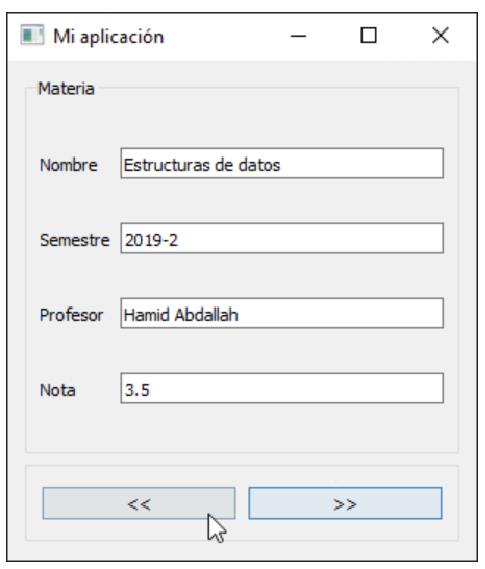
\includegraphics[width=0.4\textwidth]{Imagenes/PyQT5_Interfaz}
	\caption{Ejemplo de interfaz generada con PyQT5}
	\label{fig:interfazPYQT5}
\end{figure}

\section{Programación orientada a objetos}
La Programación Orientada a Objetos (POO) ha ganado una popularidad significativa en la comunidad de programación debido a su capacidad para desarrollar aplicaciones más robustas, flexibles y fáciles de mantener. Este paradigma se basa en la organización de programas como una colección de objetos interconectados, cada uno con su propio conjunto de datos y funcionalidades. En este artículo, exploraremos los conceptos clave de la POO, cómo implementarla en diversos lenguajes y cómo aprovechar sus ventajas para construir aplicaciones sólidas y flexibles.

La POO es un paradigma de programación que se basa en la idea de clases y objetos. Se utiliza para estructurar programas de software en piezas simples y reutilizables de código, donde una clase actúa como una plantilla para crear múltiples instancias de objetos. Este enfoque invita a considerar las entidades dentro del contexto del problema a resolver, como libros, bibliotecarios y usuarios, y representarlas como objetos con propiedades y comportamientos.

La POO se inspira en la forma en que percibimos y entendemos el mundo que nos rodea. Cada entidad se convierte en un objeto con sus propios atributos y métodos, y la interacción entre estos objetos es fundamental. La encapsulación, abstracción, herencia y polimorfismo son los principios fundamentales de la POO que permiten crear aplicaciones más organizadas, reutilizables y mantenibles.

La POO permite la reutilización del código, evita la duplicación, protege la información a través de la encapsulación y facilita el trabajo en equipo al minimizar la posibilidad de duplicar funciones. Además, proporciona una estructura más clara y modular para el desarrollo de software, lo que facilita el mantenimiento y la escalabilidad a medida que los requisitos evolucionan.

La Programación Orientada a Objetos es esencial en el diseño de aplicaciones y programas informáticos modernos. Ofrece numerosas ventajas, como la reutilización del código, la modularidad y la facilidad de mantenimiento, lo que la convierte en una opción ideal para resolver desafíos de programación complejos. Sin embargo, requiere una planificación cuidadosa y un análisis detallado de los requisitos para aprovechar al máximo sus beneficios.

\section{VPN}
\label{sec:vpn}
Claro, aquí tienes un texto más detallado y técnico sobre qué son las VPN y sus ventajas:

Una VPN (Red Privada Virtual) es una tecnología que establece una conexión segura y cifrada entre un dispositivo y una red privada remota a través de internet. Esto se logra mediante la creación de un túnel de comunicación virtual que encripta los datos transmitidos entre el dispositivo del usuario y el servidor VPN. Las VPN son utilizadas ampliamente por individuos y organizaciones para garantizar la privacidad, la seguridad y la accesibilidad de las comunicaciones en línea.

Las características y ventajas técnicas de las VPN incluyen:

Una VPN protege la privacidad al ocultar la dirección IP del usuario y encriptar los datos transmitidos. Esto previene la interceptación de datos por parte de terceros malintencionados, como hackers o agencias de vigilancia. La encriptación de extremo a extremo asegura que solo el dispositivo de origen y el servidor VPN puedan descifrar la información transmitida.

Las VPN utilizan diversos protocolos de seguridad, como IPsec (Protocolo de seguridad de Internet), SSL/TLS (Capa de sockets seguros/Protocolo de capa de transporte seguro), y OpenVPN, para establecer conexiones seguras y confiables. Estos protocolos garantizan la integridad de los datos y la autenticación de las partes involucradas en la comunicación.

Las VPN permiten a los empleados acceder de forma segura a recursos corporativos desde ubicaciones externas, utilizando conexiones cifradas. Esto es esencial para el trabajo remoto y las operaciones empresariales distribuidas, donde se necesita un acceso seguro a la red interna.

Las VPN son utilizadas por empresas para conectar múltiples ubicaciones geográficas en una red privada unificada a través de internet. Esto elimina la necesidad de redes privadas dedicadas y reduce los costos de infraestructura.

Al permitir que los usuarios simulen una ubicación diferente, las VPN facilitan el acceso a contenido y servicios en línea que podrían estar restringidos geográficamente. Esto es útil para usuarios individuales que desean acceder a sitios web o servicios que no están disponibles en su región.

Al utilizar VPN, las organizaciones pueden implementar estrategias de balanceo de carga y tolerancia a fallos para optimizar el rendimiento y la disponibilidad de sus servicios en línea.

Las VPN pueden integrarse con sistemas de filtrado de contenido y seguridad perimetral para proteger la red contra amenazas externas, como malware, phishing y ataques DDoS (denegación de servicio distribuido).


 




